% !TEX root = ../ITGO.tex

\subsection*{Speed reducer design problem}

In this problem, the total weight of the speed reducer (Figure \ref{fig:SR}) is to be minimized. The problem has seven design variables: face width ($b$), teeth module ($m$), number of teeth on the pinion ($z$), first and second length of shafts between bearings ($l_1$ and $l_2$) and first and second shafts diameter ($d_1$ and $d_2$) \citep{SR}. The problem has 11 nonlinear constraints, and the third variable is constrained to be an integer. A second version of the problem is also found in literature, where the only difference is in the lower bound of the fifth variable (7.8 for SR1 and 7.3 for SR2). The objective function value at the optimal is $f(\bm{x}^*) = 2996.34816497$ for the first version (SR1), and $f(\bm{x}^*) = 2994.471066$ for the second version (SR2). \\


\begin{figure}[h]
    \begin{center}
    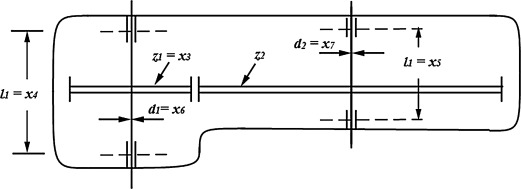
\includegraphics[scale=0.6]{Imgs/SR.jpg}
    \end{center}
    \captionsetup{justification=centering}
    \caption{Schematic view of the speed reducer design problem.}\label{fig:SR}
\end{figure}

\prob{Appendix/Problems/SR1}